% $Header$

\documentclass[t,14pt,mathserif]{beamer}

% This file is a solution template for:

% - Talk at a conference/colloquium.
% - Talk length is about 20min.
% - Style is ornate.



% Copyright 2004 by Till Tantau <tantau@users.sourceforge.net>.
%
% In principle, this file can be redistributed and/or modified under
% the terms of the GNU Public License, version 2.
%
% However, this file is supposed to be a template to be modified
% for your own needs. For this reason, if you use this file as a
% template and not specifically distribute it as part of a another
% package/program, I grant the extra permission to freely copy and
% modify this file as you see fit and even to delete this copyright
% notice. 


% Copyright 2012 by Aécio S. R. Santos <aecio.solando@gmail.com>.
%
% In principle, this file can be redistributed and/or modified under
% the terms of the GNU Public License, version 2.
%
% However, this file is supposed to be a template to be modified
% for your own needs. For this reason, if you use this file as a
% template and not specifically distribute it as part of a another
% package/program, I grant the extra permission to freely copy and
% modify this file as you see fit and even to delete this copyright
% notice. 

% Redefins a fonte
\usepackage{helvet}

% Define some colors...
\definecolor{titlecolor}{rgb}{0, 0.37, 0.59}
\definecolor{lightblue}{rgb}{.0, .68, .84}
\definecolor{black}{rgb}{0, 0, 0}
\definecolor{gray}{rgb}{0.3, 0.3, 0.3}

% Remove these comments for green color scheme
%\definecolor{titlecolor}{rgb}{0, 0.5, 0.48}
%\definecolor{lightblue}{rgb}{0.2,0.2,0.7}

% Define color of alert text
\setbeamercolor{alerted text}{fg=lightblue}

% Define tamanho das fontes
\setbeamerfont{frametitle}{parent=structure,size=\Large}
\setbeamerfont{framesubtitle}{parent=frametitle,size=\footnotesize}
\setbeamerfont{itemize/enumerate body}{size=\fontsize{16pt}{17.6pt}}
\setbeamerfont{itemize/enumerate subbody}{size=\fontsize{14pt}{15,4pt}}
\setbeamerfont{itemize/enumerate subsubbody}{size=\footnotesize}

% Redefine a fonte do titulo da capa como negrito
%\setbeamerfont{title}{size=\Large, series=\bfseries}

% Redefine cover title color
\setbeamercolor{title}{fg=titlecolor}

% Redefine title color
\setbeamercolor{frametitle}{fg=titlecolor}

% Uncomment to redefine bullets with round format
%\useinnertheme[shadow]{rounded}
%\setbeamertemplate{blocks}[rounded][shadow=\beamer@themerounded@shadow]
%\setbeamertemplate{items}[ball]

% Redefine bullets color
\setbeamercolor*{item}{fg=lightblue}

% Redefine spacing of left margin of bullets
\setlength{\leftmargini}{1.3em}
\setlength{\leftmarginii}{1em}
\setlength{\leftmarginiii}{1em}

% Redefine space between of items in 'itemize' enviroment
\newlength{\wideitemsep}
\setlength{\wideitemsep}{\itemsep}
\addtolength{\wideitemsep}{0.25pt}
\let\olditem\item
\renewcommand{\item}{\setlength{\itemsep}{\wideitemsep}\olditem}

% Redefine space before a nested itemize
\makeatletter
\def\@listii{\leftmargin\leftmarginii
              \topsep    0.9ex
              \parsep    0\p@   \@plus\p@
              \itemsep   \parsep}
\makeatother


% Redefine width of text area margins
\setbeamersize{text margin left=1em,text margin right=1em}

% Define summary items depth
\setcounter{tocdepth}{2}

% Redefine styles of frames' title
\setbeamertemplate{frametitle} {
  \vspace{0.2cm}
  \ifbeamercolorempty[bg]{frametitle}{}{\nointerlineskip}%
  \begin{beamercolorbox}[]{frametitle}
    \ifbeamercolorempty[bg]{frametitle}{}{\nointerlineskip}%
    \usebeamerfont{frametitle}{%
      \strut\insertframetitle\strut\par%
    }
    {%
      \ifx\insertframesubtitle\@empty%
      \else
  \usebeamerfont{framesubtitle}\usebeamercolor[fg]{framesubtitle}\insertframesubtitle\strut\par
      \fi
      \vspace{-.9cm}%
      {
  \textcolor{gray} {\rule[5pt]{\linewidth}{.5pt}\vspace{-8pt}}
      }
    }%  
    \vskip-0.5ex%
    \if@tempswa\else\vskip-.9cm\fi
  \end{beamercolorbox}%
  \vspace{0.2cm}
}

% Removes navigation bar
\beamertemplatenavigationsymbolsempty 

% Redefine footline to show only slide number
\setbeamertemplate{footline}{
  \begin{beamercolorbox}[wd=1\paperwidth,ht=2.25ex,dp=1ex,right]{date in head/foot}%
    %\hfill
    \insertframenumber{}                             % Only current slide number
    %\insertframenumber{} / \inserttotalframenumber  % Current slide number and total of slides
    \hspace{2ex} 
  \end{beamercolorbox}
}

%\usepackage[brazil]{babel}
\usepackage[english]{babel}

\usepackage{graphicx}	%Package para figuras
% or whatever

\usepackage[utf8]{inputenc}
% or whatever

\usepackage{times}
\usepackage[T1]{fontenc}
\usepackage{tabularx}
\usepackage{multirow}
\usepackage{adjustbox}
\usepackage{array}
%\usepackage[cmex10]{amsmath}
% Or whatever. Note that the encoding and the font should match. If T1
% does not look nice, try deleting the line with the fontenc.

\newcommand{\semitransp}[2][35]{\color{fg!#1}#2}

\title[] % (optional, use only with long paper titles)
{Evaluating the Effects of Architectural Documentation:\\
A Case Study of a Large Scale Open Source Project}

\subtitle
{Presented by Vagner Clementino}

%\author[] % (optional, use only with lots of authors)
%{Vagner Clementino~\inst{1}} %\and S.~Another\inst{2}}
% - Give the names in the same order as the appear in the paper.
% - Use the \inst{?} command only if the authors have different
%   affiliation.

\institute[] % (optional, but mostly needed)
{
%  \inst{1}%
  Department of Computer Science\\
  Federal University of Minas Gerais (UFMG)\\
  Software Archicteture - 2016\\
  %\and
  %\inst{2}%
  %Department of Theoretical Philosophy\\
  %University of Elsewhere
  }
% - Use the \inst command only if there are several affiliations.
% - Keep it simple, no one is interested in your street address.

\date[2015/04/29] %o(optional, should be abbreviation of conference name)
%{Software Quality and Measurement 2015-1 \\Prof. Eduardo Figueiredo}
% - Either use conference name or its abbreviation.
% - Not really informative to the audience, more for people (including
%   yourself) who are reading the slides online

\subject{Software Engineer}
% This is only inserted into the PDF information catalog. Can be left
% out. 



% If you have a file called "university-logo-filename.xxx", where xxx
% is a graphic format that can be processed by latex or pdflatex,
% resp., then you can add a logo as follows:

% \pgfdeclareimage[height=0.5cm]{university-logo}{university-logo-filename}
% \logo{\pgfuseimage{university-logo}}



% Delete this, if you do not want the table of contents to pop up at
% the beginning of each subsection:
\AtBeginSubsection[]
{
  \begin{frame}<beamer>{Outline}
    \tableofcontents[currentsection,currentsubsection]
  \end{frame}
}


% If you wish to uncover everything in a step-wise fashion, uncomment
% the following command: 

%\beamerdefaultoverlayspecification{<+->}

\expandafter\def\expandafter\insertshorttitle\expandafter{%
  \insertshorttitle\hfill%
  \insertframenumber\,/\,\inserttotalframenumber}

\setbeamertemplate{caption}[numbered]
\setbeamertemplate{bibliography item}{\insertbiblabel}
\begin{document}

\begin{frame}
  \titlepage
\end{frame}

\begin{frame}{Outline}
  \tableofcontents
  % You might wish to add the option [pausesections]
\end{frame}


% Structuring a talk is a difficult task and the following structure
% may not be suitable. Here are some rules that apply for this
% solution: 

% - Exactly two or three sections (other than the summary).
% - At *most* three subsections per section.
% - Talk about 30s to 2min per frame. So there should be between about
%   15 and 30 frames, all told.

% - A conference audience is likely to know very little of what you
%   are going to talk about. So *simplify*!
% - In a 20min talk, getting the main ideas across is hard
%   enough. Leave out details, even if it means being less precise than
%   you think necessary.
% - If you omit details that are vital to the proof/implementation,
%   just say so once. Everybody will be happy with that.
\section{About the Paper}

\begin{frame}{About the Paper}
	\begin{itemize}
		\item Who:
			\begin{itemize}				
				\item Kazman, Rick (Senior Member IEEE)
				\item Goldenson, Dennis (Senior Member IEEE)
				\item Monarch, Ira (Software Engineering Institute)
				\item Nichols, William (Senior Member IEEE)
				\item Valetto, Giuseppe	(Member IEEE)		
			\end{itemize}				
		\item When: 2015
		
			
	    \item Where:
	      
	       \begin{itemize}
		     
		     \item IEEE Transactions on Software Engineering  (Volume:42 ,  Issue: 3 )  
			        
	       \end{itemize}
		
	
	\end{itemize}


\end{frame}


\section{Context}

\begin{frame}{Contribution in Open Source System (OSS)}
  \begin{itemize}
  \item Sustaining large \alert{Open Source System (OSS)} requires continuos
  recruitment new participants.
  \item The number of contributors can be used as metric of project sucess.  
  \end{itemize}
\end{frame}

\begin{frame}{Objective of Architectural Documentation}
	
	\begin{itemize}
		\item Architectural documentation is believed to serve three major purposes  \cite{clements2002documenting}:		
		\begin{enumerate}
			\item providing a means of introducing new project members to the system
			\item serving as a vehicle for communication among stakeholders
			\item being the basis for system analysis and construction
		\end{enumerate}
	\end{itemize}
	
\end{frame}


\section{Motivation}

\begin{frame}{Architectural Documentation in OSS}
	
	\begin{itemize}
		\item A lack of architectural documentation might inhibit new participants since large amounts of project knowledge are unavailable to newcomers.
		\item In 5.4 percent of open source projects have any software architecture documentation \cite{6923128}
	\end{itemize}
	
\end{frame}



\section{Proposed Work}


\begin{frame}{Proposed Work}
	\begin{itemize}
	\item This is a multitrait, multimethod analysis of the effects of introducing architectural documentation into a substantial open source project
	\item The objective is to investigate \alert{if} and \alert{how} architecture documentation adds \alert{value} to a software project.
	\end{itemize}	
\end{frame}

\section{Study Design}

\begin{frame}{Open Source System Selection}
	
	\begin{itemize}
		\item The study used Hadoop Distributed File System (HDFS)\cite{shvachko2010hadoop}.
		\item The Apache Hadoop project is widely used by large companies such as Yahoo!, eBay, Facebook, and others.
	\end{itemize}
	
	\begin{figure}[!t]
		\centering
		
\includegraphics[width=3.0in]{../img/hadoop-logo}
		\label{fig:hadoop-logo}
	\end{figure}
\end{frame}


\begin{frame}{Documenting the HDFS Architecture}
	
	\begin{itemize}
		\item The architecture documentation captured the main abstractions employed in HDFS
		\item It is also to connect those abstractions to the code (files) that developers work on every day.	
	\end{itemize}

\end{frame}


\begin{frame}{HDFS Run-Time Concepts}
	\begin{figure}[!t]
		\centering
		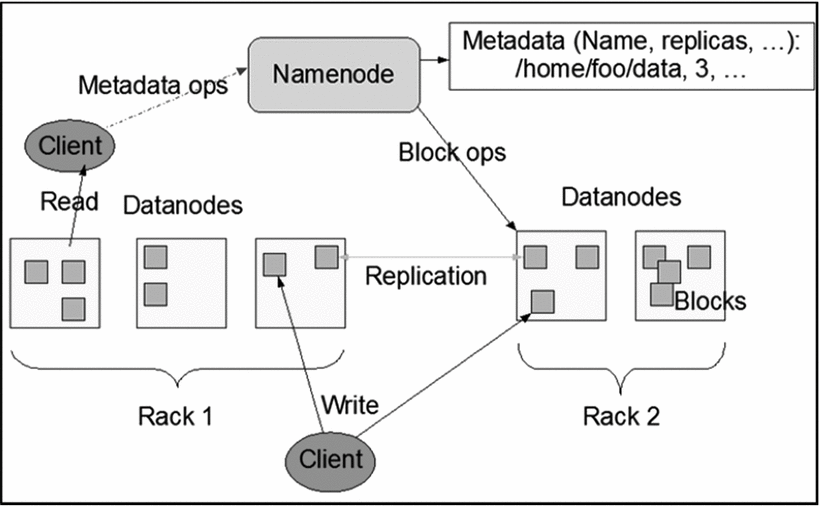
\includegraphics[width=4.5in]{../img/run-time-concept}
		\label{fig:diagrama-run-time}
	\end{figure}
\end{frame}


\begin{frame}{Documented Module Relationships in HDFS}
	\begin{figure}[!t]
		\centering
		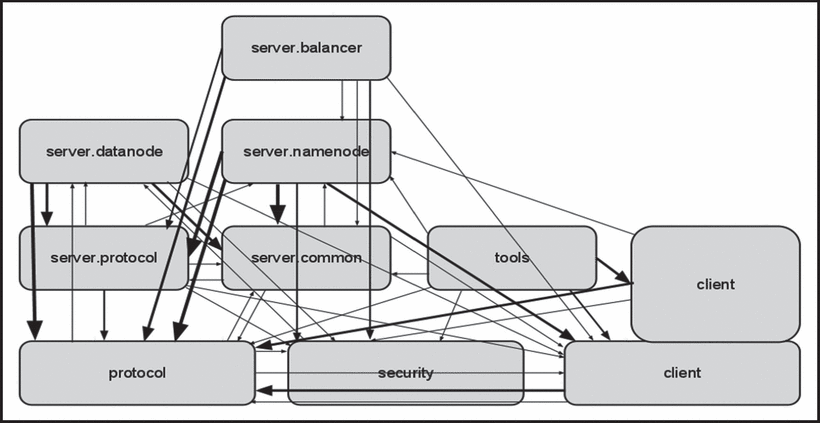
\includegraphics[width=4.5in]{../img/module-relationships}
		\label{fig:module-relationships}
	\end{figure}
\end{frame}

\begin{frame}{Research Question}
	
	\begin{description}
		\item[RQ 1.1] Was the architecture document read and if so, how much and how did it change?
		\item[RQ 1.2] Was the architecture document referred to by the project Contributors and Committers?
	\end{description}
	
\end{frame}

\begin{frame}{Research Question}
	
	\begin{description}
		\item[RQ 2.1] Was the introduction of the architecture document associated with a change in submission activity?
		\item[RQ 2.2] Was the introduction of the architecture document associated with a change in the quality of submissions?
	\end{description}
	
\end{frame}


\begin{frame}{Research Question}
	
	\begin{description}
		\item[RQ 3.1] Was the introduction of the architecture document associated with faster promotion from Commenter to Contributor to Committer?
		\item[RQ 3.2] Was the introduction of the architecture document associated with changes in project communication patterns?
	\end{description}
	
\end{frame}


\begin{frame}{Research Question}
	
	\begin{description}
		\item[RQ 4.1]  Were there any measurable differences in the use of architectural concepts in discussion of issues before and after the architecture document was introduced?
		\item[RQ 5.1] How did the Contributors and Committers use the key concepts outlined in the architecture document?
	\end{description}
	
\end{frame}


\begin{frame}{Methodology}
	

\begin{table}[!t]
	\huge
	\renewcommand{\arraystretch}{4.3}
	\resizebox{\linewidth}{2.0cm}{
			\begin{tabular}{|l|l|}
				\hline
				\multicolumn{1}{|c|}{\textbf{Research Question}} & \multicolumn{1}{c|}{\textbf{Methodology}} \\ \hline
				\textit{RQ 1.1} & Tracking how often the architecture documentation is downloaded and how often it is mentioned in discussion groups \\ \hline
				\textit{RQ 2.1 \& 2.2} & Tracking whether any changes have occurred in the interactions and activities of the HDFS developer (Contributors and Committers) \\ \hline
				\textit{RQ 3.1 \& 3.2} & Tracking project community health measures, such as the growth of the committer group, and the time lag between someone's appearance as a Contributor and their acceptance as a Committer\\ \hline
				\textit{RQ 4.1} & Tracking whether the introduction of the architecture documentation changed how the project community discussed the system \\ \hline
				\textit{RQ 2.1 \& 2.2} & Tracking product performance indicators, such as project capacity—how often Contributors made submissions to the system—and submission quality—how often submissions were rejected by the Committers \\ \hline
				\textit{RQ 1.2 \& 5.1} & Surveying the HDFS Contributor and Committer community on their opinions of the value of the architecture documentation that we created \\ \hline
			\end{tabular}
	 }

	\label{my-label}
\end{table}


\end{frame}


\section{Results}


\begin{frame}{RQ 1.1 Was the architecture document read and if so, how much and how did it change?}
	
	\begin{figure}[!t]
		\centering
		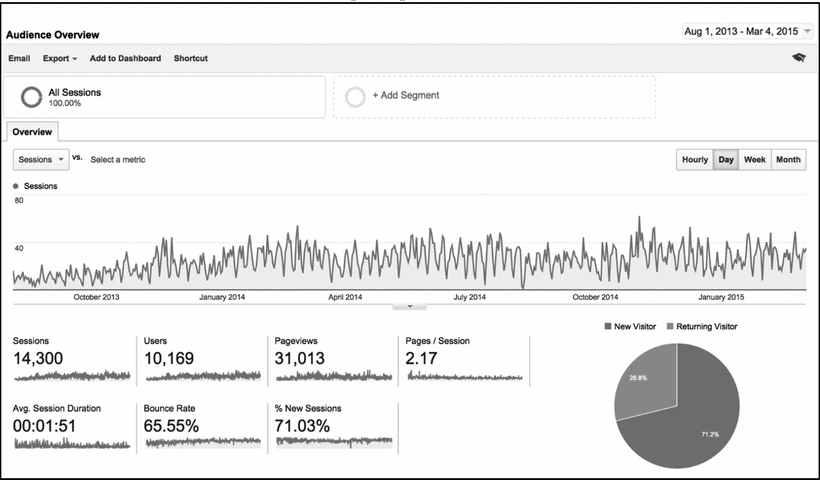
\includegraphics[width=4.0in]{../img/visitors}
		\label{fig:visitors}
	\end{figure}
		
\end{frame}


\begin{frame}{RQ 1.1 Was the architecture document read and if so, how much and how did it change?}
	
	\begin{itemize}
		\item The architecture documentation website was visited over 14,000 times in 19 months
		\item Almost 30 percent of these visits were from return visitors
		\item The access rate increased steadily during the study period.
	\end{itemize}

	
\end{frame}


\begin{frame}{RQ 1.2 Was the architecture document referred to by the project Contributors and Committers?}
	
	\begin{itemize}
		\item Based on survey the Committers and Contributors reported having made relatively little reference to the architectural document itself
		\item The HDFS Committers appeared to be beginning to advise others about the existence of the documentation available on the Internet.
	\end{itemize}

\end{frame}

\begin{frame}{RQ 2.1 Was the introduction of the architecture document associated with a change in submission activity?}
	
	\begin{figure}[!t]
		\centering
		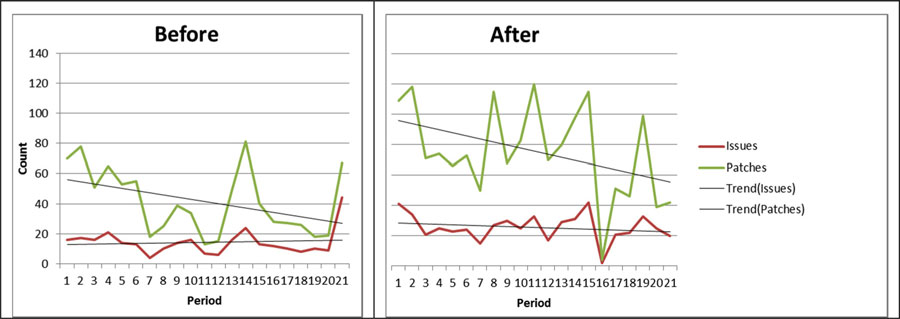
\includegraphics[width=4.0in]{../img/issue-patch}
		\label{fig:issue-patch}
	\end{figure}
	
\end{frame}


\begin{frame}{RQ 2.2 Was the introduction of the architecture document associated with a change in the quality of submissions?}
	
	\begin{figure}[!t]
		\centering
		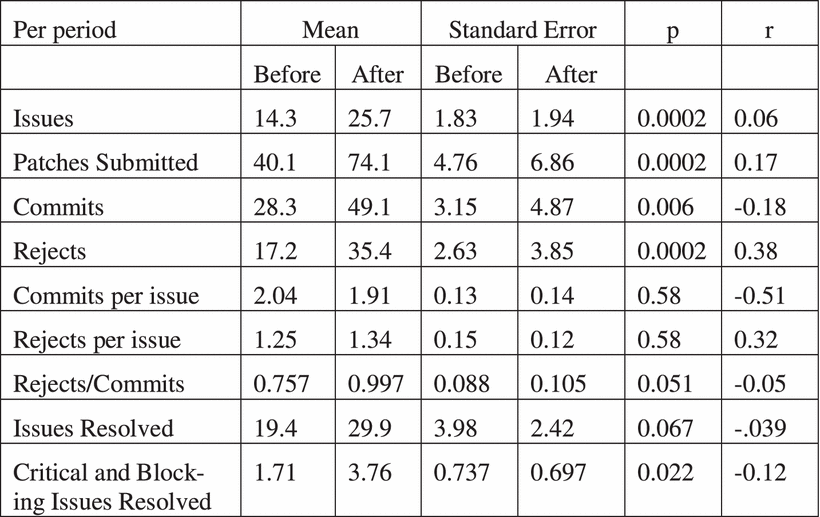
\includegraphics[width=3.0in]{../img/issue-quality-table}
		\label{fig:issue-quality-table}
	\end{figure}
	

\end{frame}



\begin{frame}{RQ 3.1 Was the introduction of the architecture document associated with faster promotion from Commenter to Contributor to Committer?}
	\begin{equation} \mathrm{Commenter} \to \mathrm{Contributor} \to \mathrm{Committer} \end{equation}

    \begin{figure}[!t]
    	\centering
    	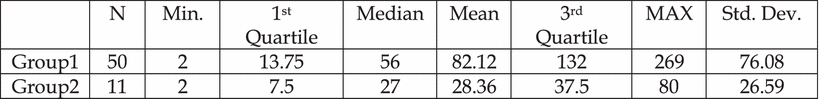
\includegraphics[width=3.0in]{../img/promotion-table}
    	\label{fig:promotion-table}
    \end{figure}
	
\end{frame}

\begin{frame}{RQ 3.2 Was the introduction of the architecture document associated with changes in project communication patterns?}
	
	\begin{figure}[!t]
		\centering
		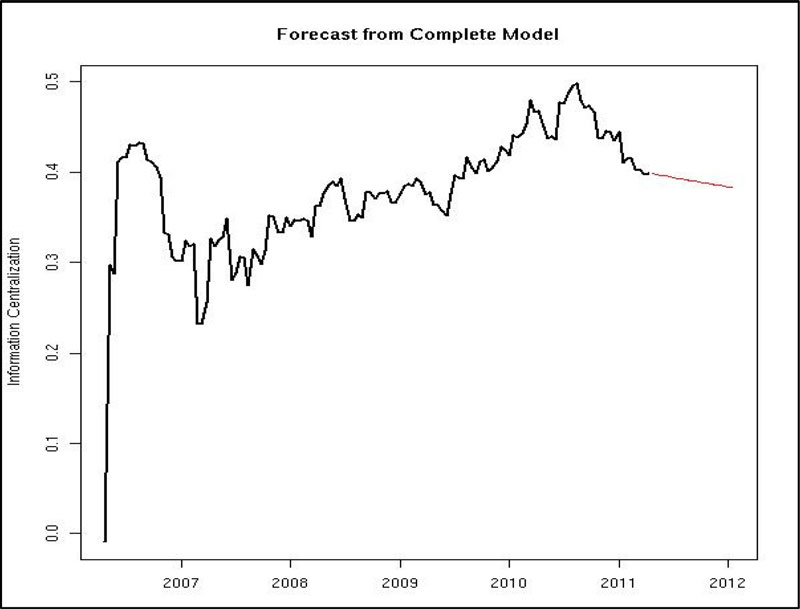
\includegraphics[width=2.5in]{../img/centrality}
		\label{fig:promotion-table}
	\end{figure}
	
\end{frame}


\begin{frame}{RQ 4.1 Were there any measurable differences in the use of architectural concepts in discussion of issues before and after the architecture document was introduced?}
	
	\begin{figure}[!t]
		\centering
		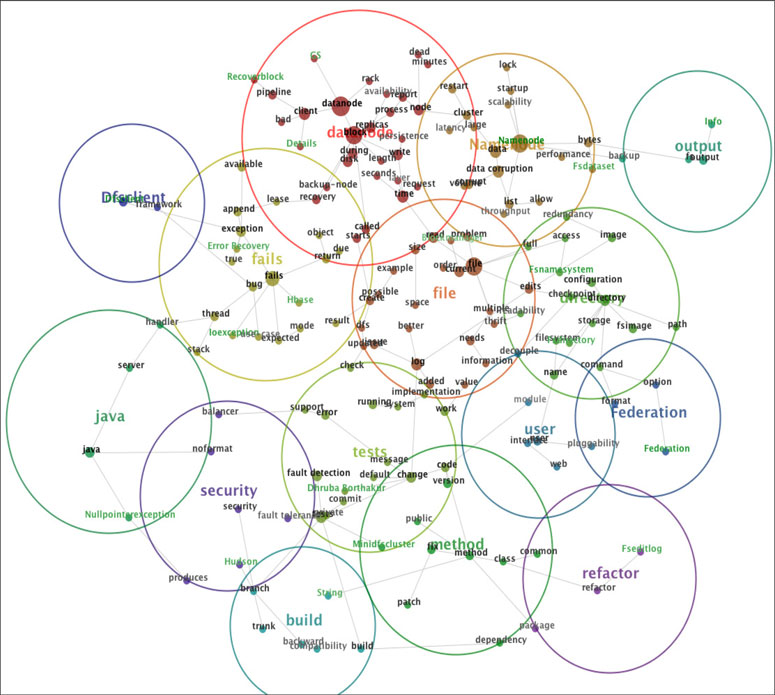
\includegraphics[width=1.9in]{../img/concept-map-before}
		\label{fig:promotion-table}
	\end{figure}
	
\end{frame}


\begin{frame}{RQ 4.1 Were there any measurable differences in the use of architectural concepts in discussion of issues before and after the architecture document was introduced?}
	
	\begin{figure}[!t]
		\centering
		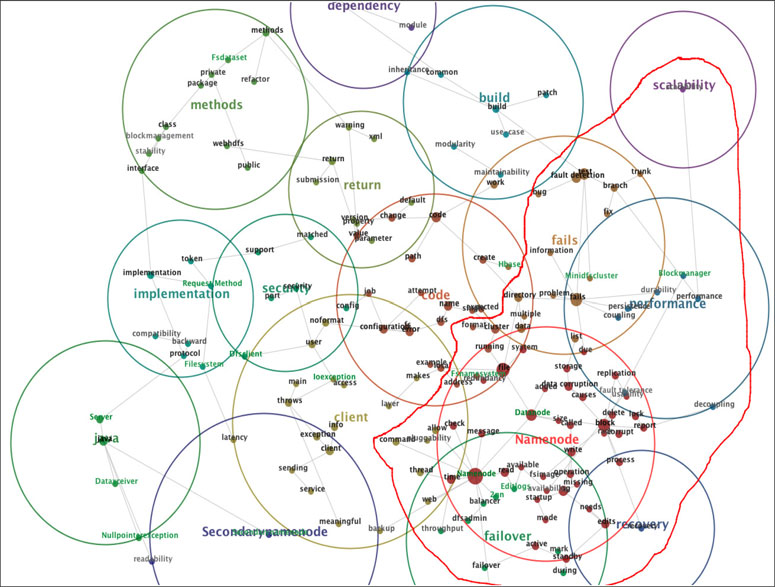
\includegraphics[width=2.0in]{../img/concept-map-after}
		\label{fig:promotion-table}
	\end{figure}
	
\end{frame}

\begin{frame}{RQ 5.1 How did the Contributors and Committers use the key concepts outlined in the architecture document?}
	\begin{itemize}
		\item Contributors and Committers we surveyed clearly recognized the importance of the concepts that were covered in the architectural document and used them in their own work on the HDFS codebase.
		\item they sometimes tended to focus more heavily on implementation details than architectural considerations \textit{per se}.		
	\end{itemize}
	
\end{frame}


\section{Conclusions}
\begin{frame}{Conclusions}
	\begin{itemize}
		\item The HDFS Committers appear to maintain intellectual control over their code base.
		\item The HDFS community of Committers and the most active Contributors is actively interested in architectural concepts.
	\end{itemize}
	
\end{frame}

\begin{frame}{Conclusions}
	\begin{itemize}
		\item The architecture documentation  to have an effect on the project, but principally on less active Contributors and newcomers.
		\item The project's social network became less centralized and the speed of promotion from Commenter to Contributor was quicker after the introduction of the documentation.
	\end{itemize}
	
\end{frame}

\section{Threats to Validity}
\begin{frame}{Threats to Validity}
	\begin{itemize}
	     \item The findings must be intended as observed correlations, whose causal linkage to architectural documentation still remains to be explored and validated
             \item :
	\end{itemize}

\end{frame}




\begin{frame}{Questions?}

	\begin{figure}[hbtp]
		\centering
	
\includegraphics[scale=1]{../img/questions.jpg}
	\end{figure}
	

\end{frame}


\begin{frame}[allowframebreaks]
   \frametitle{References}
   \bibliographystyle{IEEEtranS}
   \bibliography{IEEEfull,bibliografia}
\end{frame}

\end{document}
